%%%% Time-stamp: <2018-03-24 14:05:09 vk>
%% ========================================================================
%%%% Disclaimer
%% ========================================================================
%%
%% created by
%%
%%      Karl Voit
%%

%% ========================================================================
%%%% Basic settings
%% ========================================================================
%% (idea of using newcommands for basic documentclass settings from: Thomas Schlager)

\newcommand{\mypapersize}{A4}
%% e.g., "A4", "letter", "legal", "executive", ...
%% The size of the paper of the resulting PDF file.

\newcommand{\mylaterality}{twoside}
%% "oneside" or "twoside"
%% Either you are creating a document which is printed on both, left pages
%% and right pages (twoside) or you create a document which is printed
%% on right pages only (oneside).

\newcommand{\mydraft}{false}
%% "true" or "false"
%% Use draft mode? If true, included graphics are replaced by empty
%% rectangles (of same size) and overfull boxes (in margin space) are
%% marked with black box (-> easy to spot!)

\newcommand{\myparskip}{half}
%% e.g., "no", "full", "half", ...
%% How to separate paragraphs: indention ("no") or spacing ("half",
%% "full", ...).

\newcommand{\myBCOR}{0mm}
%% Inner binding correction. This value depends on the method which is
%% being used to bind your printed result. Some techniques do not
%% require a binding correction at all ("0mm"), other require for
%% example "5mm". Refer to KOMA script documentation for a detailed
%% explanation what a binding correction is and how to measure it.

\newcommand{\myfontsize}{12pt}
%% e.g., 10pt, 11pt, 12pt
%% The font size of the main text in pt (points).

\newcommand{\mylinespread}{1.0}
%% e.g., 1.0, 1.5, 2.0
%% Line spacing in %/100. For example 1.5 means 150% of the usual line
%% spacing. Please use with caution: 100% ("1.0") is fine because the
%% font was designed for it.

\newcommand{\mylanguage}{ngerman,american}
%% "english,ngerman", "ngerman,english", ...
%% NOTE: The *last* language is the active one!
%% See babel documentation for further details.

%% BibLaTeX-settings: (see biblatex reference for further description)
\newcommand{\mybiblatexstyle}{authoryear}
%% e.g., "alphabetic", "authoryear", ...
%% The biblatex style which is being used for referencing. See
%% biblatex documentation for further details and more values.
%%
%% CAUTION: if you change the style, please check for (in)compatible
%%          "biblatex" package options in the file
%%          "template/preamble.tex"! For example: "alphabetic" does
%%          not have an option "dashed=..." and causes an error if it
%%          does not get removed from the list of options.

\newcommand{\mybiblatexdashed}{false}  %% "true" or "false"
%% If true: replace recurring reference authors with a dash.

\newcommand{\mybiblatexbackref}{true}  %% "true" or "false"
%% If true: create backward links from reference to citations.

\newcommand{\mybiblatexfile}{references-biblatex.bib}
%% Name of the biblatex file that holds the references.

\newcommand{\mydispositioncolor}{30,103,182}
%% e.g., "30,103,182" (blue/turquois), "0,0,0" (black), ...
%% Color of the headings and so forth in RGB (red,green,blue) values.
%% NOTE: if you are using "0,0,0" for black, printers might still
%%       recognize pages as color pages. In case this is a problem
%%       (paying for color print-outs vs. paying for b/w-printouts)
%%       please edit file "template/preamble.tex" and change
%%       "\definecolor{DispositionColor}{RGB}{\mydispositioncolor}"
%%       to "\definecolor{DispositionColor}{gray}{0}" and thus
%%       overwriting the value of \mydispositioncolor above.

\newcommand{\mycolorlinks}{true}  %% "true" or "false"
%% Enables or disables colored links (hyperref package).

\newcommand{\mytitlepage}{template/title_Thesis_TU_Graz}
%% Your own or one of following pre-defined title pages:
%% "template/title_plain_maketitle": simple maketitle page
%% "template/title_Diplomarbeit_KF_Uni_Graz.tex": fancy (german) title page for KF Uni Graz
%% "template/title_Thesis_TU_Graz":
%%             titlepage for Graz University of Technology (correct
%%             (old?) Corporate Design) by Karl Voit (2012)
%% "template/title_Thesis_TU_Graz_-_kazemakase":
%%             titlepage for Graz University of Technology
%%             (correct new Corporate Design) by kazemakase (2013):
%%             see https://github.com/novoid/LaTeX-KOMA-template/issues/5
%% "template/title_VWA": titlepage for Vorwissenschaftliche Arbeit

\newcommand{\mytodonotesoptions}{}
%% e.g., "" (empty), "disable", ...
%% Options for the todonotes-package. If "disable", all todonotes will
%% be hidden (including listoftodos).

%% Load main settings for document preamble:
%% Time-stamp: <2018-03-11 14:25:47 vk>
%%%% === Disclaimer: =======================================================
%% created by
%%
%%      Karl Voit
%%
%% using GNU/Linux, GNU Emacs & LaTeX 2e
%%

%doc% %% overriding preamble/preamble.tex %%
%doc% \newcommand{\mylinespread}{1.0}  \newcommand{\mycolorlinks}{true}
%doc% \documentclass[12pt,paper=a4,parskip=half,DIV=calc,oneside,%%
%doc% headinclude,footinclude=false,open=right,bibliography=totoc]{scrartcl}
%doc% \usepackage[T1]{fontenc}\usepackage{lmodern}
%doc% \usepackage[utf8]{inputenc}\usepackage[ngerman,american]{babel}\usepackage{scrlayer-scrpage}
%doc% \usepackage{ifthen}\usepackage{eurosym}\usepackage{xspace}\usepackage[usenames,dvipsnames]{xcolor}
%doc% \usepackage[protrusion=true,factor=900]{microtype}
%doc% \usepackage{enumitem}
%doc% \usepackage[pdftex]{graphicx}
%doc% \usepackage{todonotes}
%doc% \usepackage{dingbat,bbding} %% special characters
%doc% \definecolor{DispositionColor}{RGB}{30,103,182}
%doc%
%doc% \usepackage[backend=biber,style=authoryear,dashed=false,natbib=true,hyperref=true%%
%doc% ]{biblatex}
%doc%
%doc% \addbibresource{references-biblatex.bib} %% remove, if using BibTeX instead of biblatex
%doc%
%doc% %% overriding userdata %%
%doc% \newcommand{\myauthor}{Karl Voit}\newcommand{\mytitle}{LaTeX Template Documentation}
%doc% \newcommand{\mysubject}{A Comprehensive Guide to Use the
%doc% Template from https://github.com/novoid/LaTeX-KOMA-template}
%doc% \newcommand{\mykeywords}{LaTeX, pdflatex, template, documentation, biber, biblatex}
%doc%
%doc% \newcommand{\myLaT}{\LaTeX{}@TUG\xspace}
%doc%
%doc% %% for future use?
%doc% % \usepackage{filecontents}
%doc% % \begin{filecontents}{filename.example}
%doc% %
%doc% % \end{filecontents}
%doc%
%doc%
%doc% %% using existing TeX files %%
%doc% \input{template/mycommands}
%doc% \input{template/typographic_settings}
%doc% \input{template/pdf_settings}
%doc%
%doc% \begin{document}
%doc% %% title page %%
%doc% \title{\mytitle}\subtitle{\mysubject}
%doc% \author{\myauthor}
%doc% \date{\today}
%doc%
%doc% \maketitle\newpage
%doc%
%doc% \tableofcontents\newpage
%doc% %%---------------------------------------%%

%doc%
%doc% \section{How to use this \LaTeX{} document template}
%doc%
%doc% This \LaTeX{} document template from
%doc% \myLaT\footnote{\url{http://LaTeX.TUGraz.at}} is based on \myacro{KOMA}
%doc% script\footnote{\url{http://komascript.de/}}. You don't need any
%doc% special \myacro{KOMA} knowledge (but it woun't hurt either). It provides an easy to use and
%doc% easy to modify template. All settings are documented and many references to
%doc% additional information sources are given.
%doc%

%doc% In general, there should not be any reason to modify a file in
%doc% the \texttt{template} folder. \emph{All important settings are
%doc% accessible in the main folder, mostly in the \texttt{main.tex}
%doc% file.} This way, it is easy to get what you need and you can update
%doc% the template independent of the content of the document.
%doc%
%doc% \newcommand{\myimportant}{%% mark important chapters
%doc%   \marginpar{\vspace{-1em}\rightpointleft}
%doc% }
%doc% \newcommand{\myinteresting}{\marginpar{\vspace{-2em}\PencilLeftDown}}

%doc%
%doc% The \emph{absolute minimum you should read} is listed below and
%doc% marked with the hand symbol:\myimportant
%doc% \begin{itemize}
%doc% \item Section~\ref{sec:modifytemplate}: basic configuration of this template.
%doc% \item Section~\ref{sec:howtocompile}: how to generate the \myacro{PDF} file
%doc% \item Section~\ref{sec:references}: using biblatex (instead of bibtex)
%doc% \end{itemize}
%doc%
%doc% In order to get a perfect resulting document and to get an
%doc% exciting experience with this template, you should definitely consider reading
%doc% following sections which are also marked with the pencil symbol:\myinteresting
%doc% \begin{itemize}
%doc% \item Section~\ref{sec:extending-template}: extend the template with
%doc%   your own usepackages, newcommands, and so forth
%doc% \item Section~\ref{sec:mycommands}: pre-defined commands to make your life easier (e.g., including graphics)
%doc% \item Section~\ref{sec:myacro}: how to do acronyms (like \myacro{ACME}) beautifully
%doc% \item Section~\ref{sub:csquotes}: how to \enquote{quote} text and use parentheses correctly
%doc% \end{itemize}
%doc%
%doc% The other sections describe all other settings for the sake of completeness. This is
%doc% interesting for learning more about \LaTeX{} and modifying this template to a higher level of detail.

%doc%
%doc% \newpage
%doc% \subsection{Six Steps to Customize Your Document}\myimportant
%doc% \label{sec:modifytemplate}
%doc%
%doc% This template is optimized to get to the first draft of your thesis
%doc% very quickly. Follow these instructions and you get most of your
%doc% customizing done in a few minutes:
%doc%
%doc% \newcommand{\myfile}[1]{\texttt{\href{file:#1}{#1}}}
%doc%
%doc% \begin{enumerate}
%doc% \item Modify settings in \texttt{main.tex} to meet your requirements:
%doc%   \begin{itemize}
%doc%   \item Basic settings
%doc%     \begin{itemize}
%doc%     \item Paper size, languages, font size, citation style,
%doc%           title page, and so forth
%doc%     \end{itemize}
%doc%   \item Document metadata
%doc%     \begin{itemize}
%doc%     \item Preferences like \verb+myauthor+, \verb+mytitle+, and so forth
%doc%     \end{itemize}
%doc%   \end{itemize}
%doc% \item Replace \myfile{figures/institution.pdf} with the logo of
%doc% your institution in either \myacro{PDF} or \myacro{PNG}
%doc% format.\footnote{Avoid \myacro{JPEG} format for
%doc% computer-generated (pixcel-oriented) graphics like logos or
%doc% screenshots in general. The \myacro{JEPG} format is for
%doc% photographs \emph{only}.}
%doc% \item Further down in \myfile{main.tex}:
%doc%   \begin{itemize}
%doc%   \item Create your desired structure for the chapters
%doc%         (\verb+\include{introduction}+, \verb+\include{evaluation}+, \ldots)
%doc%   \end{itemize}
%doc% \item Create the \TeX{} files and fill your content into these files you defined in the previous step.
%doc% \item Optionally: Modify \myfile{colophon.tex} to meet your situation.
%doc%   \begin{itemize}
%doc%   \item Please spend a couple of minutes and think about putting your work
%doc%         under an open license\footnote{\url{https://creativecommons.org/licenses/}}
%doc%         in order to follow the spirit of Open Science\footnote{\url{https://en.wikipedia.org/wiki/Open_science}}.
%doc%   \end{itemize}
%doc% \item In case you are using \myacro{GNU} make\footnote{If you
%doc%       don't know, what \myacro{GNU} make is, you are not using it (yet).}:
%doc%       Put your desired \myacro{PDF} file name in the second line of file
%doc%    \myfile{Makefile}
%doc%    \begin{itemize}
%doc%    \item replace \enquote{Projectname} with your filename
%doc%    \item do not use any file extension like \texttt{.tex} or \texttt{.pdf}
%doc%    \end{itemize}
%doc% \end{enumerate}
%doc%
%doc%

%doc%
%doc% \subsection{License}\myimportant
%doc% \label{sec:license}
%doc%
%doc% This template is licensed under a Creative Commons Attribution-ShareAlike 3.0 Unported (CC BY-SA 3.0)
%doc%         license\footnote{\url{https://creativecommons.org/licenses/by-sa/3.0/}}:
%doc%     \begin{itemize}
%doc%     \item You can share (to copy, distribute and transmit) this template.
%doc%     \item You can remix (adapt) this template.
%doc%     \item You can make commercial use of the template.
%doc%     \item In case you modify this template and share the derived
%doc%           template: You must attribute the template such that you do not
%doc%           remove (co-)authorship of Karl Voit and you must not remove
%doc%           the URL to the original repository on
%doc%           github\footnote{\url{https://github.com/novoid/LaTeX-KOMA-template}}.
%doc%     \item If you alter, transform, or build a new template upon
%doc%           this template, you may distribute the resulting
%doc%           template only under the same or similar license to this one.
%doc%     \item There are \emph{no restrictions} of any kind, however, related to the
%doc%           resulting (PDF) document!
%doc%     \item You may remove the colophon (but it's not recommended).
%doc%     \end{itemize}


%doc%
%doc%
%doc% \subsection{How to compile this document}\myimportant
%doc% \label{sec:howtocompile}
%doc%
%doc% I assume that compiling \LaTeX{} documents within your software
%doc% environment is something you have already learned. This template is
%doc% almost like any other \LaTeX{} document except it uses
%doc% state-of-the-art tools for generating things like the list of
%doc% references using biblatex/biber (see
%doc% Section~\ref{sec:references} for details). Unfortunately, some \LaTeX{} editors
%doc% do not support this much better way of working with bibliography
%doc% references yet. This section describes how to compile this template.
%doc%
%doc% \subsubsection{Compiling Using a \LaTeX{} Editor}
%doc%
%doc% Please do select \myfile{main.tex} as the \enquote{main project file} or make
%doc% sure to compile/run only \myfile{main.tex} (and not \myfile{introduction.tex}
%doc% or other \TeX{} files of this template).
%doc%
%doc% Choose \texttt{biber} for generating the references. Modern LaTeX{}
%doc% environments offer this option. Older tools might not be that up to
%doc% date yet.
%doc%

%doc% \subsubsection{Activating \texttt{biber} in the \LaTeX{} editor TeXworks}
%doc% \label{sec:biberTeXworks}
%doc%
%doc% The \href{https://www.tug.org/texworks/}{TeXworks} editor is a very
%doc% basic (but fine) \LaTeX{} editor to start with. It is included in
%doc% \href{http://miktex.org/}{MiKTeX} and
%doc% \href{http://miktex.org/portable}{MiKTeX portable} and supports
%doc% \href{https://en.wikipedia.org/wiki/Syntax_highlighting}{syntax
%doc%   highlighting} and
%doc% \href{http://itexmac.sourceforge.net/SyncTeX.html}{SyncTeX} to
%doc% synchronize \myacro{PDF} output and \LaTeX{} source code.
%doc%
%doc% Unfortunately, TeXworks shipped with MiKTeX does not support compiling
%doc% using \texttt{biber} (biblatex) out of the box. Here is a solution to
%doc% this issue. Go to TeXworks: \texttt{Edit} $\rightarrow$
%doc% \texttt{Preferences~\ldots} $\rightarrow$ \texttt{Typesetting} $\rightarrow$
%doc% \texttt{Processing tools} and add a new entry (using the plus icon):
%doc%
%doc% \begin{tabbing}
%doc%   Arguments: \= foobar  \kill
%doc%   Name:      \> \verb#pdflatex+biber# \\
%doc%   Program:   \> \emph{find the \texttt{template/pdflatex+biber.bat} file from your disk} \\
%doc%   Arguments: \> \verb+$fullname+ \\
%doc%              \> \verb+$basename+
%doc% \end{tabbing}
%doc%
%doc% Activate the \enquote{View PDF after running} option.
%doc%
%doc% Close the preferences dialog and you will now have an additional
%doc% choice in the drop down list for compiling your document. Choose the
%doc% new entry called \verb#pdflatex+biber# and start a happier life with
%doc% \texttt{biber}.
%doc%
%doc% In case your TeXworks has a German user interface, here the key
%doc% aspects in German as well:
%doc%
%doc% \begin{otherlanguage}{ngerman}
%doc%
%doc%   \texttt{Bearbeiten} $\rightarrow$ \texttt{Einstellungen~\ldots} $\rightarrow$
%doc%   \texttt{Textsatz} $\rightarrow$ \texttt{Verarbeitungsprogramme} $\rightarrow$
%doc%   + \emph{(neues Verarbeitungsprogramm)}:
%doc%
%doc% \begin{tabbing}
%doc%   Befehl/Datei: \= foobar  \kill
%doc%     Name: \> pdflatex+biber \\
%doc%     Befehl/Datei: \> \emph{die \texttt{template/pdflatex+biber.bat} im Laufwerk suchen} \\
%doc%     Argumente: \> \verb+$fullname+ \\
%doc%                \> \verb+$basename+
%doc% \end{tabbing}
%doc%
%doc% \enquote{PDF nach Beendigung anzeigen} aktivieren.
%doc%
%doc% \end{otherlanguage}
%doc%

%doc% \subsubsection{Compiling Using \myacro{GNU} make}
%doc%
%doc% With \myacro{GNU}
%doc% make\footnote{\url{https://secure.wikimedia.org/wikipedia/en/wiki/Make\_\%28software\%29}}
%doc% it is just simple as that: \texttt{make pdf}
%doc%
%doc% Several other targets are available. You can check them out by
%doc% executing: \texttt{make help}
%doc%
%doc% In case you are using TeXLive (instead of MiKTeX as I do), you might
%doc% want to modify the line \texttt{PDFLATEX\_CMD = pdflatex} within
%doc% the file \texttt{Makefile} to: \texttt{PDFLATEX\_CMD = pdflatex -synctex=1 -undump=pdflatex}
%doc%
%doc%

%doc% \subsubsection{Compiling in a Text-Shell}
%doc%
%doc% To generate a document using \texttt{Biber}, you can stick to
%doc% following example:
%doc% \begin{verbatim}
%doc% pdflatex main.tex
%doc% biber main
%doc% pdflatex main.tex
%doc% pdflatex main.tex
%doc% \end{verbatim}
%doc%
%doc% Users of TeXLive with Microsoft Windows might want to try the
%doc% following script\footnote{Thanks to Florian Brucker for provinding
%doc%   this script.} which could be stored as, e.g., \texttt{compile.bat}:
%doc% \begin{verbatim}
%doc% REM call pdflatex using parameters suitable for TeXLive:
%doc% pdflatex.exe  "main.tex"
%doc% REM generate the references metadata for biblatex (using biber):
%doc% biber.exe "main"
%doc% REM call pdflatex twice to compile the references and finalize PDF:
%doc% pdflatex.exe  "main.tex"
%doc% pdflatex.exe -synctex=-1 -interaction=nonstopmode "main.tex"
%doc% \end{verbatim}
%doc%


%doc%
%doc% \subsection{How to get rid of the template documentation}
%doc%
%doc% Simply remove the files \verb#Template_Documentation.pdf# and
%doc% \verb#Template_Documentation.tex# (if it exists) in the main folder
%doc% of this template.
%doc%
%doc% \subsection{What about modifying or extending the template?}\myinteresting
%doc% \label{sec:extending-template}
%doc%
%doc% This template provides an easy to start \LaTeX{} document template with sound
%doc% default settings. You can modify each setting any time. It is recommended that
%doc% you are familiar with the documentation of the command whose settings you want
%doc% to modify.
%doc%
%doc% It is recommended that for \emph{adding} things to the preambel (newcommands,
%doc% setting variables, defining headers, \dots) you should use the file
%doc% \texttt{main.tex}.
%doc% There are comment lines which help you find the right spot.
%doc% This way you still have the chance to update your \texttt{template}
%doc% folder from the template repository without losing your own added things.
%doc%
%doc% The following sections describe the settings and commands of this template and
%doc% give a short overview of its features.

%doc% \subsection{How to change the title page}
%doc%
%doc% This template comes with a variety of title pages. They are located in
%doc% the folder \texttt{template}. You can switch to a specific title
%doc% page by including the corresponding title page file in the file
%doc% \texttt{main.tex}.
%doc%
%doc% Please note that you may not need to modify any title page document by
%doc% yourself since all relevant information is defined in the file
%doc% \texttt{main.tex}.

%doc%
%doc% \section{\texttt{preamble.tex} --- Main preamble file}
%doc%
%doc% In the file \verb#preamble/preamble.tex# you will find the basic
%doc% definitions related to your document. This template uses the \myacro{KOMA} script
%doc% extension package of \LaTeX{}.
%doc%
%doc% There are comments added to the \verb#\documentclass{}# definitions. Please
%doc% refer to the great documentation of \myacro{KOMA}\footnote{\texttt{scrguide.pdf} for
%doc% German users} for further details.
%doc%
%doc% \paragraph{What should I do with this file?} For standard purposes you might
%doc% use the default values it provides. You must not remove its \texttt{include} command
%doc% in \texttt{main.tex} since it contains important definitions. This file contains
%doc% settings which are documented well and can be modified according to your needs.
%doc% It is recommended that you fully understand each setting you modify in order to
%doc% get a good document result. However, you can set basic values in the
%doc% \texttt{main.tex} file: font size, paper size,
%doc% paragraph separation mode, draft mode, binding correction, and whether
%doc% your document will be a one sided document or you are planning to
%doc% create a document which is printed on both, left side and right side.
%doc%

\documentclass[%
fontsize=\myfontsize,%% size of the main text
paper=\mypapersize,  %% paper format
parskip=\myparskip,  %% vertical space between paragraphs (instead of indenting first par-line)
DIV=calc,            %% calculates a good DIV value for type area; 66 characters/line is great
headinclude=true,    %% is header part of margin space or part of page content?
footinclude=false,   %% is footer part of margin space or part of page content?
open=right,          %% "right" or "left": start new chapter on right or left page
appendixprefix=true, %% adds appendix prefix; only for book-classes with \backmatter
bibliography=totoc,  %% adds the bibliography to table of contents (without number)
draft=\mydraft,      %% if true: included graphics are omitted and black boxes
                     %%          mark overfull boxes in margin space
BCOR=\myBCOR,        %% binding correction (depends on how you bind
                     %% the resulting printout.
\mylaterality        %% oneside: document is not printed on left and right sides, only right side
                     %% twoside: document is printed on left and right sides
]{scrbook}  %% article class of KOMA: "scrartcl", "scrreprt", or "scrbook".
            %% CAUTION: If documentclass will be changed, *many* other things
            %%          change as well like heading structure, ...

% ADDED MANUALLY!
\usepackage{colortbl}
%

% FIXXME: adopting class usage:
% from scrbook -> scrartcl OR scrreport:
% - remove appendixprefix from class options
% - remove \frontmatter \mainmatter \backmatter \appendix from main.tex

% FIXXME: adopting language:
% add or modify language parameter of package »babel« and use language switches described in babel-documentation

%doc%
%doc% \subsection{\texttt{fontenc}: Switch to Western European output charset}
%doc%
%doc% This allows \LaTeX{} to output special digits like german mutated vovels or quotation marks without assembling them of basic US-ASCII ones. This makes text in the generated pdf copyable. Sadly this also influences the fonts used, as the default ones do not contain most of the characters we use here. The lmodern font set is usually used to counteract this problem.
%doc%
\usepackage[T1]{fontenc}
\usepackage{lmodern}
%% Source: https://texwelt.de/fragen/5537/was-macht-eigentlich-usepackaget1fontenc
%%         https://tex.stackexchange.com/questions/227063/fontenc-changes-sans-serif-bold-font-in-koma-script

%doc%
%doc% \subsection{\texttt{inputenc}: UTF8 as input charset}
%doc%
%doc% You are able and should use \myacro{UTF8} character settings for writing these \TeX{}-files.
%doc%
%\usepackage{ucs}             %% UTF8 as input characters; UCS incompatible to biblatex
\usepackage[utf8]{inputenc} %% UTF8 as input characters
%% Source: http://latex.tugraz.at/latex/tutorial#laden_von_paketen

%doc%
%doc% \subsection{\texttt{textcomp}: Support for Text Companion fonts}
%doc%
%doc% Provides some text symbols such as bullet in \myacro{TS1} encoding.
%doc% Depending on what font or symbols you use, you might not even need this.
%doc% Removing this package will at worst result in a warning.
\usepackage{textcomp}
%% Source: https://www.ctan.org/pkg/textcomp

%doc%
%doc% \subsection{\texttt{babel}: Language settings}
%doc%
%doc% The default setting of the language is American. Please change settings for
%doc% additional or alternative languages used in \texttt{main.tex}.
%doc%
%doc% Please note that the default language of the document is the \emph{last} language
%doc% which is added to the package options.
%doc%
%doc% To set only parts of your document in a different language as the rest, use for example\newline
%doc% \verb+\foreignlanguage{ngerman}{Beispieltext in deutscher Sprache}+\newline
%doc% For using foreign language quotes, please refer to the \verb+\foreignquote+,
%doc% \verb+\foreigntextquote+, or \verb+\foreignblockquote+ provided by
%doc% \texttt{csquotes} (see Section~\ref{sub:csquotes}).
%doc%
\usepackage[\mylanguage]{babel}  %% used languages; default language is *last* language of options

%doc%
%doc% \subsection{\texttt{scrlayer-scrpage}: Headers and footers}
%doc%
%doc% Since this template is based on \myacro{KOMA} script it uses its great
%doc% \texttt{scrlayer-scrpage} (previously \texttt{scrpage2})
%doc% package for defining header and footer information. Please refer to the \myacro{KOMA}
%doc% script documentation how to use this package.
%doc%
\usepackage{scrlayer-scrpage} %%  advanced page style using KOMA


%doc%
%doc% \subsection{References}\myimportant
%doc% \label{sec:references}
%doc%
%doc% This template is using
%doc% \href{http://www.tex.ac.uk/tex-archive/info/translations/biblatex/de/}{\texttt{biblatex}}
%doc% and \href{http://en.wikipedia.org/wiki/Biber_(LaTeX)}{\texttt{Biber}}
%doc% instead of
%doc% \href{http://en.wikipedia.org/wiki/BibTeX}{\textsc{Bib}\TeX{}}. This has the following
%doc% advantages:
%doc% \begin{itemize}
%doc% \item better documentation
%doc% \item Unicode-support like German umlauts (ö, ä, ü, ß) for references
%doc% \item flexible definition of citation styles
%doc% \item multiple bibliographies e.\,g. for printed and online resources
%doc% \item cleaner reference definition e.\,g. inheriting information from
%doc%   \texttt{Proceedings} to all related \texttt{InProceedings}
%doc% \item modern implementation
%doc% \end{itemize}
%doc%
%doc% In short, \texttt{biblatex} is able to handle your \texttt{bib}-files
%doc% and offers additional features. To get the most out of
%doc% \texttt{biblatex}, you should read the very good package
%doc% documentation. Be warned: you'll probably never want to change back
%doc% to \textsc{Bib}\TeX{} again.
%doc%
%doc% Take a look at the files \texttt{references-bibtex.bib} and
%doc% \texttt{references-biblatex.bib}: they contain the three
%doc% references \texttt{tagstore}, \texttt{Voit2009}, and
%doc% \texttt{Voit2011}.
%doc% The second file is optimized for \texttt{biblatex} and
%doc% takes advantage of some features that are not possible with
%doc% \textsc{Bib}\TeX{}.
%doc%
%doc% This template is ready to use \texttt{biblatex} with \texttt{Biber} as
%doc% reference compiler. You should make sure that you have installed an up
%doc% to date binary of \texttt{Biber} from its
%doc% homepage\footnote{\url{http://biblatex-biber.sourceforge.net/}}.
%doc%
%doc%
%doc% In \texttt{main.tex} you can define several general \texttt{biblatex}
%doc% options: citation style, whether or not multiple occurrences of
%doc% authors are replaced with dashes, or if backward references (from
%doc% references to citations) should be added.
%doc%
%doc%
%doc% If you are using the LaTeX{} editor TeXworks, please make sure that
%doc% you have read Section~\ref{sec:biberTeXworks} in order to use
%doc% \texttt{biber}.
%doc%

%doc% \subsubsection{Example citation commands}
%doc%
%doc% This section demonstrates some example citations using the style \texttt{authoryear}.
%doc% You can change the citation style in \texttt{main.tex} (\texttt{mybiblatexstyle}).
%doc%
%doc% \begin{itemize}
%doc% \item cite \cite{Eijkhout2008} and cite \cite{Bringhurst1993, Eijkhout2008}.
%doc% \item citet \citet{Eijkhout2008} and citet \citet{Bringhurst1993, Eijkhout2008}.
%doc% \item autocite \autocite{Eijkhout2008} and autocite \autocite{Bringhurst1993, Eijkhout2008}.
%doc% \item autocites \autocites{Eijkhout2008} and autocites \autocites{Bringhurst1993, Eijkhout2008}.
%doc% \item citeauthor \citeauthor{Eijkhout2008} and citeauthor \citeauthor{Bringhurst1993, Eijkhout2008}.
%doc% \item citetitle \citetitle{Eijkhout2008} and citetitle \citetitle{Bringhurst1993, Eijkhout2008}.
%doc% \item citeyear \citeyear{Eijkhout2008} and citeyear \citeyear{Bringhurst1993, Eijkhout2008}.
%doc% \item textcite \textcite{Eijkhout2008} and textcite \textcite{Bringhurst1993, Eijkhout2008}.
%doc% \item smartcite \smartcite{Eijkhout2008} and smartcite \smartcite{Bringhurst1993, Eijkhout2008}.
%doc% \item footcite \footcite{Eijkhout2008} and footcite \footcite{Bringhurst1993, Eijkhout2008}.
%doc% \item footcite with page \footcite[p.42]{Eijkhout2008} and footcite with page \footcite[compare][p.\,42]{Eijkhout2008}.
%doc% \item fullcite \fullcite{Eijkhout2008} and fullcite \fullcite{Bringhurst1993, Eijkhout2008}.
%doc% \end{itemize}
%doc%
%doc% Please note that the citation style as well as the bibliography style
%doc% can be changed very easily. Refer to the settings in
%doc% \texttt{main.tex} as well as the very good documentation of \texttt{biblatex}.
%doc%

%doc% \subsubsection{Using this template with \myacro{APA} style}
%doc%
%doc% First, you have to have the \myacro{APA} biblatex style
%doc% installed. Modern \LaTeX{} distributions do come with
%doc% \texttt{biblatex} and \myacro{APA} style. If so, you will find the
%doc% files \texttt{biblatex-apa.pdf} (style documentation) and
%doc% \texttt{biblatex-apa-test.pdf} (file with citation examples) on your
%doc% hard disk.
%doc%
%doc% \begin{enumerate}
%doc% \item Change the style according to \verb#\newcommand{\mybiblatexstyle}{apa}#
%doc% \item Add \verb#\DeclareLanguageMapping{american}{american-apa}# or \\
%doc%   \verb#\DeclareLanguageMapping{german}{german-apa}# to your
%doc%   preamble\footnote{You might want to use section \enquote{MISC
%doc%       self-defined commands and settings} for this.}
%doc% \end{enumerate}
%doc%
%doc% These steps change the biblatex style to \myacro{APA} style

%doc%
%doc% \subsubsection{Using this template with \textsc{Bib}\TeX{}}
%doc%
%doc% If you do not want to use \texttt{Biber} and \texttt{biblatex}, you
%doc% have to change several things:
%doc% \begin{itemize}
%doc% \item in \verb#preamble/preamble.tex#
%doc%   \begin{itemize}
%doc%   \item remove the usepackage command of \texttt{biblatex}
%doc%   \item remove the \verb#\addbibresource{...}# command
%doc%   \end{itemize}
%doc% \item in \verb#main.tex#
%doc%   \begin{itemize}
%doc%   \item replace \verb=\printbibliography= with the usual
%doc%     \verb=\bibliographystyle{yourstyle}= and \verb=\bibliography{yourbibfile}=
%doc%   \end{itemize}
%doc% \item if you are using \myacro{GNU} \texttt{make}: modify \verb=Makefile=
%doc%   \begin{itemize}
%doc%   \item replace \verb#BIBTEX_CMD = biber# with \verb#BIBTEX_CMD = bibtex#
%doc%   \end{itemize}
%doc% \item Use the reference file \texttt{references-bibtex.bib}
%doc%   instead of \texttt{references-biblatex.bib}
%doc% \end{itemize}
%doc%
%doc%
\usepackage[backend=biber, %% using "biber" to compile references (instead of "biblatex")
%style=\mybiblatexstyle, %% see biblatex documentation
style=numeric, %% see biblatex documentation
%dashed=\mybiblatexdashed, %% do *not* replace recurring reference authors with a dash
backref=\mybiblatexbackref, %% create backlings from references to citations
natbib=true, %% offering natbib-compatible commands
hyperref=true, %% using hyperref-package references
]{biblatex}  %% remove, if using BibTeX instead of biblatex

\addbibresource{\mybiblatexfile} %% remove, if using BibTeX instead of biblatex



%doc%
%doc% \subsection{Miscellaneous packages} \label{subsec:miscpackages}
%doc%
%doc% There are several packages included by default. You might want to activate or
%doc% deactivate them according to your requirements:
%doc%
%doc% \begin{enumerate}

%doc% \item[\texttt{\href{http://ctan.org/pkg/ifthen}{%%
%doc% ifthen%%
%doc% }}]
%doc% For using if/then/else statements for example in macros
\usepackage{ifthen}

%doc% \item[\texttt{\href{http://www.ctan.org/pkg/graphicx}{%%
%doc% graphicx%%
%doc% }}]
%doc% The widely used package to use graphical images within a \LaTeX{} document.
\ifthenelse{\boolean{\mydraft}}{   %% the \mydraft switches between
                                   %% showing rectangles instead of graphics
  \usepackage[pdftex,draft]{graphicx}
}
{
  \usepackage[pdftex]{graphicx}
}

%doc% \item[\texttt{\href{https://secure.wikimedia.org/wikibooks/en/wiki/LaTeX/Formatting\#Other\_symbols}{%%
%doc% pifont%%
%doc% }}]
%doc% For additional special characters available by \verb#\ding{}#
\usepackage{pifont}

%% pre-define ifthen-boolean variables:
\newboolean{myaddcolophon}
\newboolean{myaddlistoftodos}
\newboolean{english_affidavit}


%doc% \item[\texttt{\href{http://www.ctan.org/tex-archive/fonts/eurosym}{%%
%doc% eurosym%%
%doc% }}]
%doc% Using the character for Euro with \verb#\officialeuro{}#
%\usepackage{eurosym}

%doc% \item[\texttt{\href{http://www.ctan.org/tex-archive/help/Catalogue/entries/xspace.html}{%%
%doc% xspace%%
%doc% }}]
%doc% This package is required for intelligent spacing after commands
\usepackage{xspace}

%doc% \item[\texttt{\href{https://secure.wikimedia.org/wikibooks/en/wiki/LaTeX/Colors}{%%
%doc% xcolor%%
%doc% }}]
%doc% This package defines basic colors. If you want to get rid of colored links and headings
%doc% please change corresponding value in \texttt{main.tex} to \{0,0,0\}.
\usepackage[usenames,dvipsnames]{xcolor}
\definecolor{DispositionColor}{RGB}{\mydispositioncolor} %% used for links and so forth in screen-version

%doc% \item[\texttt{\href{http://www.ctan.org/pkg/ulem}{%%
%doc% ulem%%
%doc% }}]
%doc% This package offers strikethrough command \verb+\sout{foobar}+.
\usepackage[normalem]{ulem}

%doc% \item[\texttt{\href{http://www.ctan.org/pkg/framed}{%%
%doc% framed%%
%doc% }}]
%doc% Create framed, shaded, or differently highlighted regions that can
%doc% break across pages.  The environments defined are
%doc% \begin{itemize}
%doc%   \item framed: ordinary frame box (\verb+\fbox+) with edge at margin
%doc%   \item shaded: shaded background (\verb+\colorbox+) bleeding into margin
%doc%   \item snugshade: similar
%doc%   \item leftbar: thick vertical line in left margin
%doc% \end{itemize}
\usepackage{framed}

%doc% \item[\texttt{\href{http://www.ctan.org/pkg/eso-pic}{%%
%doc% eso-pic%%
%doc% }}]
%doc% For example on title pages you might want to have a logo on the upper right corner of
%doc% the first page (only). The package \texttt{eso-pic} is able to place things on absolute
%doc% and relative positions on the whole page.
\usepackage{eso-pic}

%doc% \item[\texttt{\href{http://ctan.org/pkg/enumitem}{%%
%doc% enumitem%%
%doc% }}]
%doc% This package replaces the built-in definitions for enumerate, itemize and description.
%doc% With \texttt{enumitem} the user has more control over the layout of those environments.
\usepackage{enumitem}

%doc% \item[\texttt{\href{http://www.ctan.org/tex-archive/macros/latex/contrib/todonotes/}{%%
%doc% todonotes%%
%doc% }}]
%doc% This packages is \emph{very} handy to add notes\footnote{\texttt{todonotes} replaced
%doc% the \texttt{fixxme}-command which previously was defined in the
%doc% \texttt{preamble\_mycommands.tex} file.}. Using for example \verb#\todo{check}#
%doc% results in something like this \todo{check} in the document. Do read the
%doc% great package documentation for usage of other very helpful commands such as
%doc% \verb#\missingfigure{}# and \verb#\listoftodos#. The latter one creates an index of all
%doc% open todos which is very useful for getting an overview of open issues.
%doc% The package \texttt{todonotes} require the packages \texttt{ifthen}, \texttt{xkeyval}, \texttt{xcolor},
%doc% \texttt{tikz}, \texttt{calc}, and \texttt{graphicx}. Activate
%doc% and configure \verb#\listoftodos# in \texttt{main.tex}.
%\usepackage{todonotes}
\usepackage[\mytodonotesoptions]{todonotes}  %% option "disable" removes all todonotes output from resulting document

%disabled% \item[\texttt{\href{http://www.ctan.org/tex-archive/macros/latex/contrib/blindtext}{%%
%disabled% blindtext%%
%disabled% }}]
%disabled% This package is used to generate blind text for demonstration purposes.
%disabled% %% This is undocumented due to problems using american english; author informed
%disabled% \usepackage{blindtext}  %% provides commands for blind text:
%disabled% %% \blindtext creates some text,
%disabled% %% \Blindtext creates more text.
%disabled% %% \blinddocument creates a small document with sections, lists...
%disabled% %% \Blinddocument creates a large document with sections, lists...
%% 2012-03-10: vk: author published a corrected version which is able to handle "american english" as well. Did not have time to check new package version for this template here.

%doc% \item[\texttt{\href{http://ctan.org/tex-archive/macros/latex/contrib/units}{%%
%doc% units%%
%doc% }}]
%doc% For setting correctly typesetted units and nice fractions with \verb+\unit[42]{m}+ and \verb+\unitfrac[100]{km}{h}+.
\usepackage{units}


%doc% \end{enumerate}




%%%% End
%%% Local Variables:
%%% TeX-master: "../main"
%%% mode: latex
%%% mode: auto-fill
%%% mode: flyspell
%%% eval: (ispell-change-dictionary "en_US")
%%% End:
%% vim:foldmethod=expr
%% vim:fde=getline(v\:lnum)=~'^%%%%'?0\:getline(v\:lnum)=~'^%doc.*\ .\\%(sub\\)\\?section{.\\+'?'>1'\:'1':
%% DO NOT REMOVE THIS LINE!

\setboolean{myaddcolophon}{true}  %% "true" or "false"
%% If set to "true": a colophon (with notes about this document
%% template, LaTeX, ...) is added after the title page.
%% Please do not set to "false" without a good reason. The colophon
%% helps your readers to get in touch with LaTeX and to find this template.

\setboolean{myaddlistoftodos}{false}  %% "true" or "false"
%% If set to "true": the current list of open todos is added after the
%% table of contents. If \mytodonotesoptions is set to "disable", no
%% list of todos is added, independent of this setting here.

\setboolean{english_affidavit}{true}  %% "true" or "false"
%% If set to "true": the language of the statutory declaration text is set to
%% English, otherwise it is in German.


%% ========================================================================
%%%% Document metadata
%% ========================================================================

%% general metadata:
\newcommand{\myauthor}{AUTHOR}  %% also used for PDF metadata (hyperref)
\newcommand{\myauthorwithexistingtitles}{\myauthor{}, OLDDEGREE}  %% including
                                %% university degree already held
                                %% (BSc, MSc, ...)
\newcommand{\mytitle}{TITLE}  %% also used for PDF metadata (hyperref)
\newcommand{\mysubtitle}{ }  %% only used with title_Thesis_TU_Graz_-_kazemakase
\newcommand{\mysubject}{SUBJECT}  %% also used for PDF metadata (hyperref)
\newcommand{\mykeywords}{KEYWORDS}  %% also used for PDF metadata (hyperref)

%% this information is used only for generating the title page:
\newcommand{\myworktitle}{Master's Thesis}  %% official type of work like ``Master theses''
\newcommand{\mygrade}{Master of Science} %% title you are getting with this work like ``Master of ...''
\newcommand{\mystudy}{Telematik} %% your study like ``Arts''
\newcommand{\mydegreeprogramme}{Master's degree programme: \mystudy} %% Master's or PhD degree programme
\newcommand{\myuniversity}{Graz University of Technology} %% your university/school
\newcommand{\myfaculty}{ }  %% only used with title_Thesis_TU_Graz_-_kazemakase
\newcommand{\myinstitute}{Institute for Softwaretechnology} %% affiliation
\newcommand{\myinstitutehead}{Univ.-Prof.\,Dipl-Ing.\,Dr.techn.~Some One} %% head of institute
\newcommand{\mysupervisor}{Dr.~Some Body} %% your supervisor
\newcommand{\mycosupervisor}{\ }  %% only used with title_Thesis_TU_Graz_-_kazemakase
\newcommand{\myevaluator}{Prof.~Some Genius} %% your evaluator
\newcommand{\myhomestreet}{Street~42} %% your home street (with house number)
\newcommand{\myhometown}{Graz} %% your home town
\newcommand{\myhomepostalnumber}{8010} %% your postal number of home town
\newcommand{\mysubmissionmonth}{November} %% month you are handing in
\newcommand{\mysubmissionyear}{2013} %% year you are handing in
\newcommand{\mysubmissiontown}{\myhometown} %% town of handing in (or \myhometown)


%% additional information for generic_documentation title page
\newcommand{\myid}{1234567} %% Matrikelnummer
\newcommand{\mylecture}{LECTURE} %%


%% ========================================================================
%%%% MISC command definitions
%% ========================================================================
\input{template/mycommands}

%% ========================================================================
%%%% Typographic settings
%% ========================================================================
\input{template/typographic_settings}


%% ========================================================================
%%%% MISC usepackages
%% ========================================================================

%% ... it's OK to put here your own usepackage commands ...




%% ========================================================================
%%%% MISC self-defined commands and settings
%% ========================================================================

%% ... it's OK to put here your own newcommand/newenvironment-definitions ...




\newcommand{\myLaT}{\LaTeX{}@TUG\xspace} %% LaTeX@TUG text "logo"

\hyphenation{ex-am-ple hy-phen-ate}  %% in order to use German umlauts
%% here (Ver-\"of-fent-li-chung), you have to check for
%% activated \usepackage[T1]{fontenc} in the preamble

%% override default language of babel: (be sure to know, what you're
%% doing here)
%\selectlanguage{american}
%\selectlanguage{ngerman}

%% ========================================================================
%%%% Templates
%% ========================================================================

%% template for inserting figures:
% \myfig{}%% filename
%       {}%% width/height
%       {}%% caption
%       {}%% optional (short) caption for list of figures
%       {fig:}%% label

%% acronyms in small caps: \myacro{UNESCO}


\input{template/pdf_settings}  %% should be *last* definitions in preamble!
%% ========================================================================
%%%% begin{document}
%% ========================================================================
\begin{document}

\frontmatter                    %% KOMA: roman page numbers and such; only available in scrbook

\input{colophon}                %% defines information about editor, LaTeX, font, ...

%% Choose your desired title page:
\input{\mytitlepage}            %% include title page


\input{template/declaration_TU_Graz}  %% Statutory Declaration
% \input{thanks}                %% this is a suggestion: you have to create this file on demand
% \input{foreword}              %% this is a suggestion: you have to create this file on demand


%% include the abstract without chapter number but include it on table of contents:
\cleardoublepage
\phantomsection
\addcontentsline{toc}{chapter}{Abstract}
\include{abstract}              %% Abstract


\tableofcontents                %% this produces the table of contents - you might have guessed :-)

\listoffigures

%% if myaddlistoftodos is set to "true", the current list of open todos is added:
\ifthenelse{\boolean{myaddlistoftodos}}{
  \newpage\listoftodos          %% handy if you are using todonotes with \todo{}
}{}                             %% with todonotes-package option "disable" you can get rid of any todo in the output

\mainmatter                     %% KOMA: marks main part using arabic page numbers and such; only available in scrbook


% \input{example-short-chapter}   %% remove this line to get rid of the example chapter
% \input{example-style-chapter}   %% remove this line to get rid of the style chapter

%% include tex file chapters:
\chapter{Introduction}
Automated driving has made considerable advancements in the last 15 years, yet significant technical challenges still persist~\cite{ayoub_manual_2019}.
Fully developed and integrated, it will have a lasting impact on mobility, road safety and society at large~\cite{milakis_policy_2017}.

Automated driving systems are considered safety-critical and need responsible and thorough testing in order to mitigate traffic accidents and human harm. As outlined by \cite{kluck_search-based_2022}, the main requirements of automated driving systems are that they "must operate under all circumstances" and, crucially, "must be safe". Self-driving systems have the potential for harm, as their failure may lead to catastrophic accidents. Errors can be difficult to detect, due to the complexity of the environment, in which automated driving systems operate. High quality testing is subsequently needed in order to ensure safety on the road. 

\begin{quote}
	\begin{em}
		\enquote{Thoroughly validating and verifying automated or autonomous driving functions is inevitable for assuring to meet quality criteria for safety-critical systems.}~\cite{felbinger_comparing_2019}
	\end{em}
\end{quote}

According to \cite{kalra_driving_2016}, achieving statistical safety for autonomous driving systems necessitates a significant number of miles driven. Accumulating this amount might not be feasible by driving solely in the real world. \cite{kluck_search-based_2022} adds, that unguided mileage collection may provide only "limited quality assurance". During real world driving, the number of challenging situations is low, given most everyday situations can be driven without trouble.

Different complexity levels of driving automation are defined by \cite{saej3016} with a level 5 system being required to perform the entire task of diving completely without a human driver. Lower levels take over only parts of the driving, such as parking and steering. Examples include driver support features such as Automatic Emergency Braking (AEB) or Automatic Lane Keep Systems (ALKS). Testing these lower levels is similarly vital.

According to \cite{kluck_search-based_2022}, search based testing (SBT) is a valuable tool for improving the robustness and revealing systematic failures of automated driving systems. SBT generates inputs for a system under test in order to provoke some unwanted behaviour. It utilizes a problem-specific cost function that guides the search towards areas that have a high probability of failures. SBT can be applied to complex and large search spaces, where other, less focused, testing tools like full factorial or random testing might struggle.

Genetic algorithms (GAs) are a viable tool of search based testing and were already successfully utilized in the domain of automated driving, as evidenced by notable studies \cite{klampfl_using_nodate, felbinger_comparing_2019, kaufmann_critical_2021, almanee_scenorita_2021}. This master's thesis will employ a genetic algorithm in order to generate critical driving scenarios for testing self-driving technology in vehicles. While generating these scenarios is the objective, the main task of the thesis will evolve around the implementation of the genetic algorithm as well as the optimization of its hyperparameters. In the following chapters, the vehicle under test is refereed to as 'EGO' vehicle, while all other road users are denoted as 'NPCs'.

\section{Research Questions}
The following two research questions will provide a guideline for this master's thesis. Both questions evolve around examining and comparing the performance of a genetic algorithm on generating critical scenarios for autonomous vehicles. The specifics of the actual cost function are explained in Chapter \ref{chap:implementation}.

\subsection{Research Question 1}
\begin{quote}
	\begin{em}
		\textit{Is a genetic algorithm suitable for generating critical driving scenarios compared to random search?}
	\end{em}
\end{quote}

While the mentioned papers provide strong suggestions that a genetic algorithm has a significant advantages over random search, a direct comparison is still crucial important. Are situations where a genetic algorithm struggles to find critical scenarios compared to a random search approach?

\subsection{Research Question 2}
\begin{quote}
	\begin{em}
		\textit{Can the performance of a genetic algorithm be improved by optimizing the control parameter using the taguchi method?}
	\end{em}
\end{quote}

To tune the hyperparameter of the genetic algorithm, design of experiment, specifically the Taguchi method, was employed. In an effort to test, if significant performance improvements are possible, the optimized GA will be compared to a GA using control parameters as recommended by existing literature. This evaluation aims to understand, whether  the Taguchi method can indeed lead to notable performance advancements for genetic algorithms.
























\chapter{Tools}
\section{Genetic Algorithm}

While a short intrododuction was already given, the idea of a Genetic Algorithm will now be explained in greater detail.
We will have a look at its History and then discussing the most important parameters.

\todo{Usage of GA}

\subsection{History}
The GA was invented by....


\subsection{Different Hyperparameter}
Hyperparamter have a huge influence on the performance of a Genetic Algorihm. They have an impact on the "convergin" ...
It has been shown, that there is no universal hyperparamter set and that it needs to be optimized on a per "problem" basis.

\subsubsection{Num of generations}
The Number of Generation defines the duration of a GA. As long as the algorihtm has not converged, ....?
For my testing, using a generation size of 40 was almost always sufficient, and will thus mostly be used.

\subsubsection{Pop Size}
Pop size will set the number of Individuals of a GA per Generation. The higher the pop size, the bigger the less change of premature converging. 
It will however also lead to a longer convergin time.

\subsubsection{Selection}
Selection defines how which individuals are allowed to mate and move into the next generation.

\todo{pros and cons of roulette vs Tournament}
tournament was chosen to be used for this works because of this paper (and also because of pros and cons list)

Other ideas are evolve around having a flexible selection system debending on fitness \todo{cite paper}

\subsubsection{Crossover}
Crossover is the mating process.
\todo{Discuss all used crossover methods}


\subsubsection{Mutation}
Mutation is responsible for introducing new information into the gene pool.

\todo{Discuss individual mutation}
\todo{Discuss all used mutation methods}

\subsubsection{Other}
More to come....

\section{Behavior Tree}
A behavior tree is a decision tree. \todo{insert a good introduction to BT}

\subsection{Usage for GA}
Due to the fact, \todo{insert ref to discussion}, that there is no full stack available for the EGO vehicle, a solution had to be found.
In order to have the Genetic Algorithm controll only NPCs and not the EGO vehicle itselve, a behaviour tree is used.
The behaviour tree is used to controll the EGO vehicle over the action interface provided by the Traffic Manager. This is the same as the Genetic Algorithm is doing.

The behaviour tree will define which direction the EGO should take at junctions and it will realistically dodge obstacles intoduced by the Genetic Algorithm. The main goal of the BT is to make the EGO vehicle behave in a realistic way.

In a further chapter it will be dicussed if a GA with controll of the EGO (i.e. no BT will be used) lead to better cost.



\chapter{Implementation}

\section{Traffic Manager}
A custom developed Traffic Manger will be used to simulate an environment, that can subsequently be controlled by the Genetic Algorithm. The Traffic Manager is not part of this thesis and will be regarded as a "blackbox", only recieving a brief introduction.
In general, it will simulate traffic starting from a predefined scenarios which defines the positions and types of vehicles and pedestrians(i.e. actors). 
A simulation always consist of at least one EGO vehicle. Additionally any number of NPCs can be used.

While the NPCs are only controlled by the Traffic Manager, the ego vehicle can be either partly or completely controlled by an ADAS/AD function. The goal of the Genetic Algorithm is to test these functions for safety.

For all simulations done by this thesis, the Traffic Manager was set to 100Hz and the simulation duration set to 35 seconds.

\subsection{Action Interface}
\label{implementation:action_interface}
To control the behaviour of the actors inside the simulation, actions can be requested over the "Action Interface", which is provided by the Traffic Manager. An action will initiate a certain behaviour from an actor. It can be set to at any timestep for any actor\footnote{depending on the ADAS/AD function under test, the Action Interface might be disabled for the EGO vehicle}. Pedestrians and vehicles have a different set of actions.

\todo{Insert graph of action interface}

If no action is set, the actor will behave in a normal manner inside the simulation. This means that the actor will follow along its path until a new action changes its behaviour.

The following list are all actions provided by the traffic manager that were available for the genetic algorithm at the time of this master thesis.
\begin{itemize}
	\item JunctionSelection
	\begin{itemize}
		\item Parameters: Vehicle ID: int, Junction\_selection\_angle: float
		\item Angle is set in radiant. Default value is 0. Vehicles will chose which direction to take at a junction based on this angle.
	\end{itemize}
	\item LaneChange
	\begin{itemize}
		\item Parameters: Vehicle ID: int, ...
		\item Initiates a LaneChange based on its given parameters.
	\end{itemize}
	\item AbortLaneChange
	\begin{itemize}
		\item Parameters: Vehicle ID: int, ...
		\item If a LaneChange is currently happening, it will get aborted.
	\end{itemize}
	\item ModifyTargetVelocity
	\begin{itemize}
		\item Parameters: Vehicle ID: int, ...
		\item Modifies the interal Target Velocity of the Traffic Manager by a percentage. If it is for example 0, the vehicle will stop.
	\end{itemize}
	\item TurnHeading
	\begin{itemize}
		\item Parameters: Pedestrian ID: int, ...
		\item The pedestrian will turn 180 degrees and walk in the oposite direction
	\end{itemize}
	\item CrossRoad
	\begin{itemize}
		\item Parameters: Pedestrian ID: int, ...
		\item The pedestrian will cross the road immediately.
	\end{itemize}
	\item CrossAtCrosswalk
	\begin{itemize}
		\item Parameters: Pedestrian ID: int, ...
		\item The pedestrian will cross the road at the next crosswalk.
	\end{itemize}
\end{itemize}

All these actions are accessed by the Genetic Algorithm and the Behavior tree. The Behaviour tree sets only actions for the EGO vehicle, while the Genetic Algorithm will set all actions for the other actors in the simulation.

\subsection{Map and Starting Scenario}
The map is Town10 from Carla. It was chosen, because 1. its roads are self contained, 2. its not too big, yet still complex and 3. its supported by Carla and thus visualization looks better.

The Starting Scenario defines the number and type of all actors as well as their position. It needs to be created manually.



\section{Genetic Algorithm}
The task of the Genetic Algorithm is to search for sequences of actions that will result in the most interesting scenarios according to its cost function.
For implementing the Genetic Algorithm, DEAP\footnote{\url{https://deap.readthedocs.io/en/master}} was chosen. It is a popular tool for academia and allows for high customisability.
As has been stated in section \ref{implementation:action_interface}, the algorithm has full access over setting actions for all NPCs. Searching for sequences of actions, it tries to optimize a cost function. This section aims to explain how the genetic algorithm was implemented and which different hyperparameters are variable. In chapter \ref{chap:hyperparameter_tuning}, the best hyperparameter combination will be generated, further analysis is done in \ref{chap:evaluation}.

A few default settings for the genetic algorithm had to be chosen. It was decided that the genetic algorithm will set an action per actor every 50 steps, which translates to 0.5 seconds (simulation runs at 100hz). In other words, every 50 steps of the simulation is 1 timestep for the genetic algorithm. The time of a simulation is always set to 35 seconds. Each genetic algorithm will run for 30 generations. These to settings were chosen with the aim of reducing the amount of needed computations.

If the GA decides to not set an action for the integer, it sets "NoAction" as a placeholder.

\subsection{Usage for GA}
\todo{maybe remove}
Due to the fact, \todo{insert ref to discussion}, that there is no full stack available for the EGO vehicle, a solution had to be found.
In order to have the Genetic Algorithm control only NPCs and not the EGO vehicle itselve, a behaviour tree is used.
The behaviour tree is used to control the EGO vehicle over the action interface provided by the Traffic Manager. This is the same as the Genetic Algorithm is doing.

The behaviour tree will define which direction the EGO should take at junctions and it will realistically dodge obstacles intoduced by the Genetic Algorithm. The main goal of the BT is to make the EGO vehicle behave in a realistic way.


\subsection{Encoding}
When implementing a Genetic Algorithm, it is necessary to implement an encoding that fits to the problem. Each individual basically thus needs to include all actions that the genetic algorithm wants to apply. Different encodings presented in section \ref{chap:foundation:ga:encoding}, however none directly fitted to the problem presented. A custom encoding for both chromosomes and genes needed to be generated.

\subsubsection{Chromosome}
Each individual has 1 chomosome which consits of a list of genes, which has been explained in section \todo{ref}. Starting out, 2 different encodings came to mind, in both cases, the genes position in the chromosome defined the time an action is set.

\paragraph{Time}
The first encoding is will be called "Time". Each gene corresponds to 1 timestep (so 1 gene per every 0.5 seconds). One gene has a list of the length of the number of all NPCs. This list is populated with actions. The index of an action in the list corresponds to the NPC id (index + 1 as the ego has id == 0, thus a start at 1 is needed). A visualization is seen in figure \ref{figure:encoding:chromosome:time}.

\begin{figure}[ht] 
	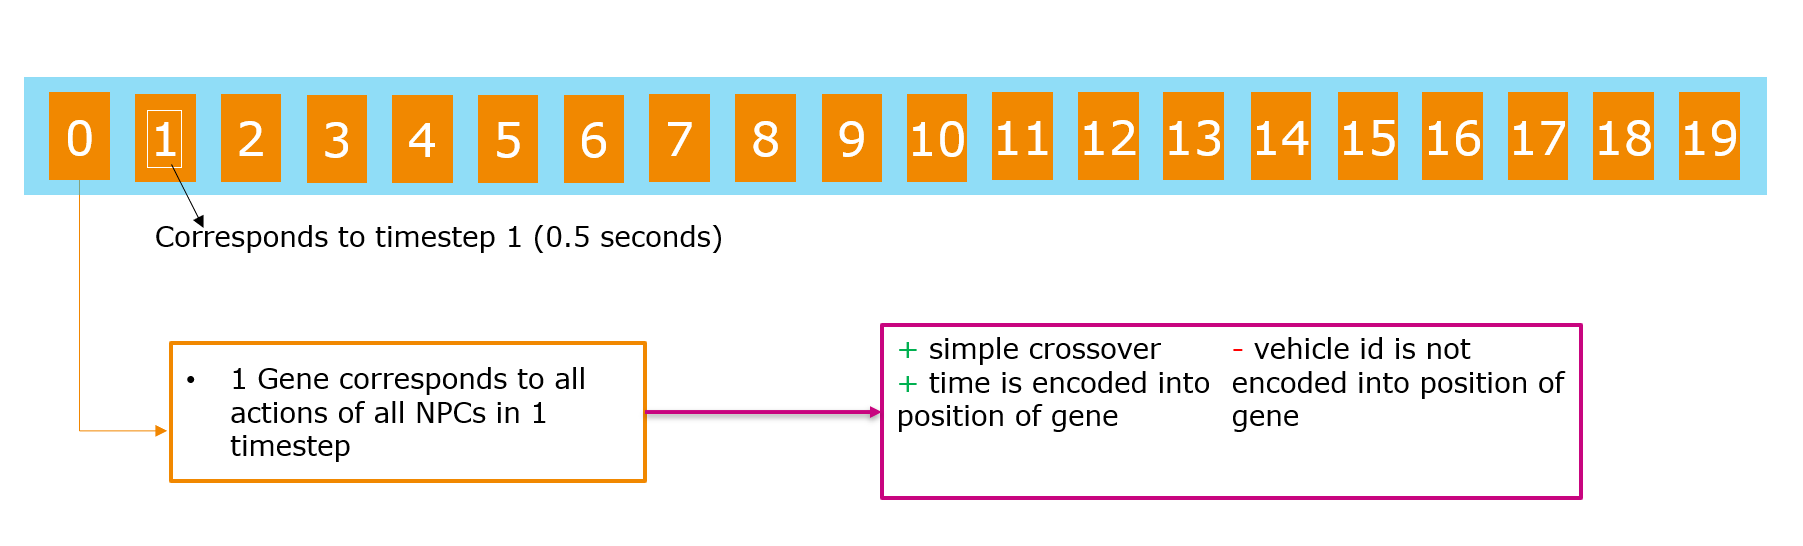
\includegraphics[width=1\linewidth]{figures/time_encoding}
	\caption{Time}
	\label{figure:encoding:chromosome:time}
\end{figure}


Given the previously stated simulation time of 35 seconds, each chromosome has a length of $35 * 2 = 70$ genes. Each gene consits of $number\_of\_actors$ actions.
Crossover can thus only move all actions of a timestep at once, modifing between actions of the same timestep can only be done using mutation. If this is desired will be seen in the next chapters.


\paragraph{TimeNPC}
The second encoding has the name "TimeNPC", and is somewhat differently structured. Now, genes only hold 1 action, encoding now not only the timestep, but also the actor id in the position of the gene inside the chromosome. Now, each actors actions will be listed one after another. This is visualized in figure \ref{figure:encoding:chromosome:time_npc}.

\begin{figure}[ht] 
	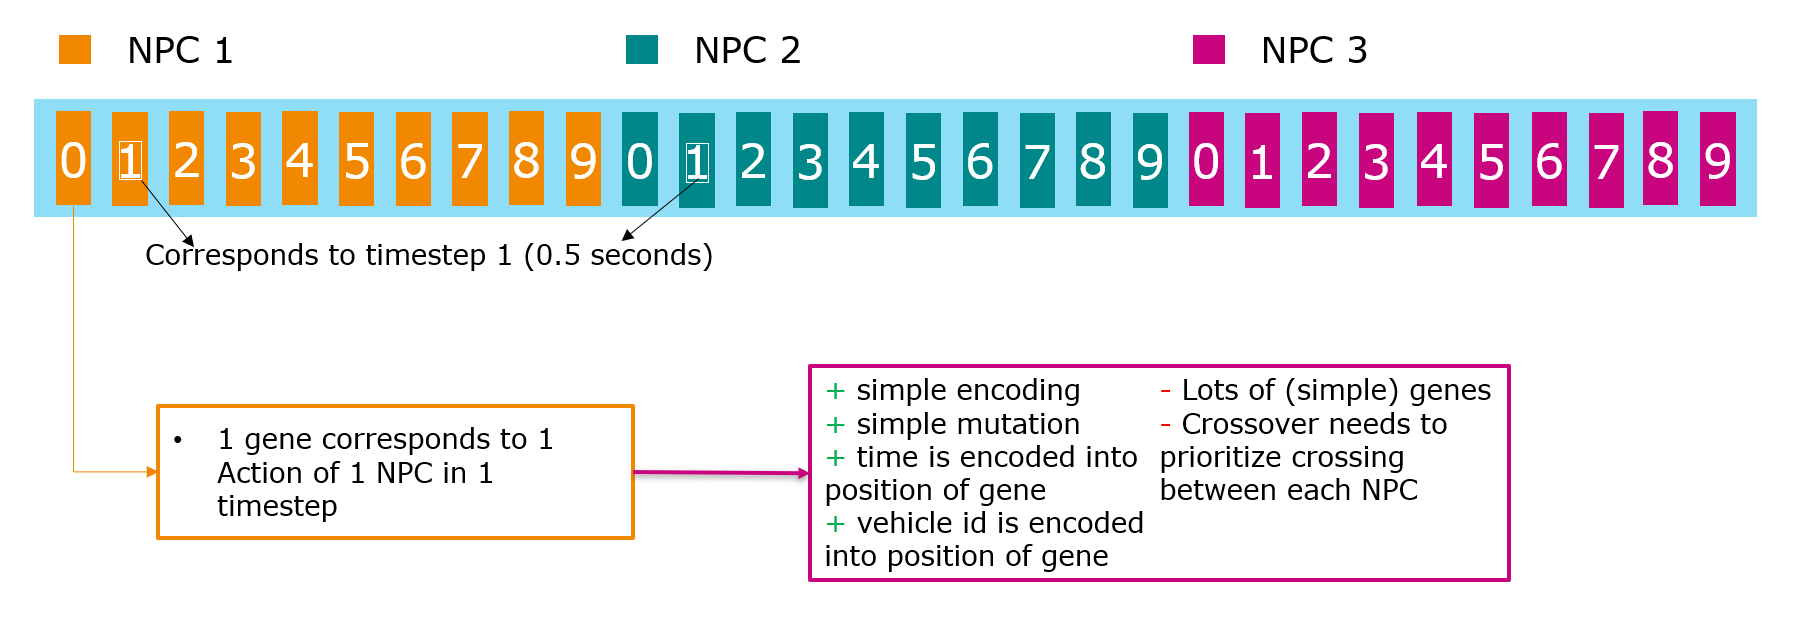
\includegraphics[width=1\linewidth]{figures/time_npc_encoding}
	\caption{Time + NPC}
	\label{figure:encoding:chromosome:time_npc}
\end{figure}

Now, each gene has a length of $1$ and each chromosome now has a length of $35 * 2 * number\_of\_actors$, which makes them much longer compared to the previous encoding. This now allows the crossover operation to modify only specific actions of one timesstep. Previously this was not possible.

However for this encoding to make sense, the crossover operations "OnePoint" and "TwoPoint" had to be modified as follows. In an example of 10 NPCs, the operations will be executed for each NPC separately. Otherwise these two operations would have only had an effect on 1 or 2 different NPCs. For the reaiming NPCs, their actions would stay the same.

\subsubsection{Gene}
Two different encodings for genes were implemented as well. A gene always consits of a list, which depending on the chromosome type either has a length of $number\_of\_actors$ (In case ChromosomeEncoding == Time) or of length 1 (in case ChromosomeEncoding == TimeNPC). The following two encodings thus show the type of object, which is in these lists.

\paragraph{Integer}
The first encoding uses integer, which are translated into actions when the simulation is started. For each action, a range of integers is assigned, the larger the range, the more likely the action is chosen by the GA. Actions that have parameters are split into different ranges, according to which paramters make sense. For example ModifyTargetVelocity is split into five different parts, with different percentages, namely 50, 70, 100, 130, 160. The range of integers assigned to these parts is different. A percentage setting of 100 for example has the largest integer range assigned.
In Appendix , the probabilty of an actions can be seen. In Appendix ... the probabitly per actions of the parameters can be viewed.

These ranges were assigned based on intuition and trial and error. The encoding is visualized in \ref{figure:encoding:gene:int}.

TODO: Due to the cliff problem, it was decided to not use binary representations for these integers. Due to the mutation choosing the integers randomly, it is not a problem that the variables are not really "continous".

\begin{figure}[ht] 
	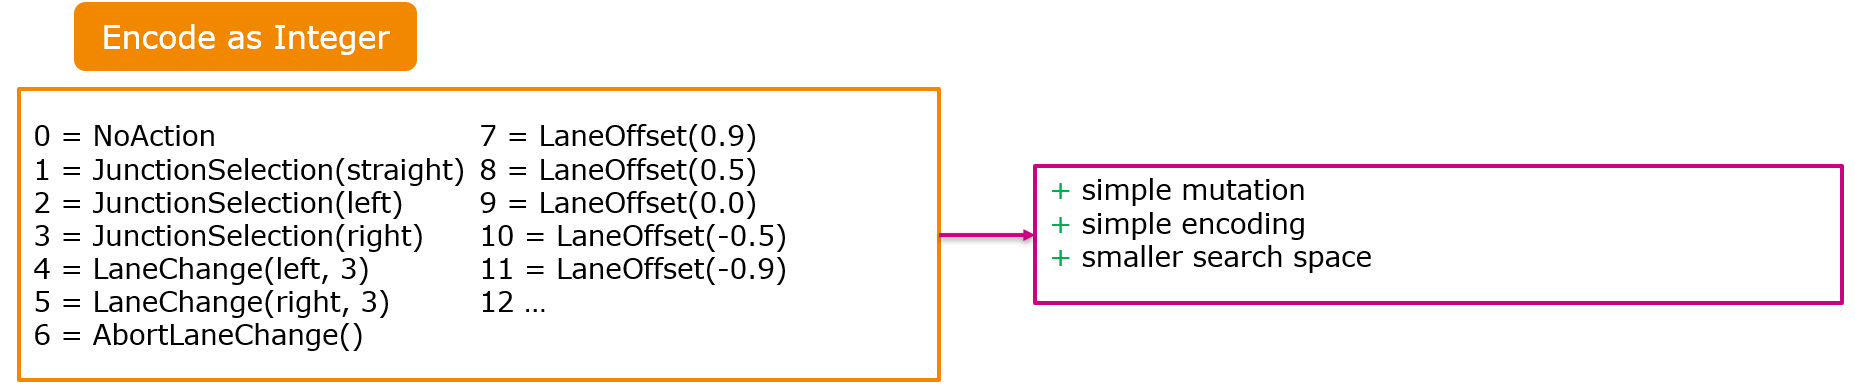
\includegraphics[width=1\linewidth]{figures/int_encoding}
	\caption{Integer}
	\label{figure:encoding:gene:int}
\end{figure}

\paragraph{Dictionary}
The second encoding is much similar to the actual actions used in the simulations. Now, no translation is necessary anymore. During generation of the individuals, each action is again selected based on different probabilities assigned to actions, which again can be viewed in Appendix ... . These probablilites are the same as for the integer encoding. However the difference is, in case an action has parameters that need to be chosen. 
For each parameter, a range and a randomness function was chosen. For example in case of the percenetage parameter in ModifyTargetVelocity, the values are selected from a GausDistribution, with mu= 100, sigma=25 and a range limit between 0 and 300.

Again, these probability functions with settings were assigned based on intuition as well as trial and error. Detailed information can be seen in Appendix...

Figure \ref{figure:encoding:gene:dict} shows a visualization.

\begin{figure}[ht] 
	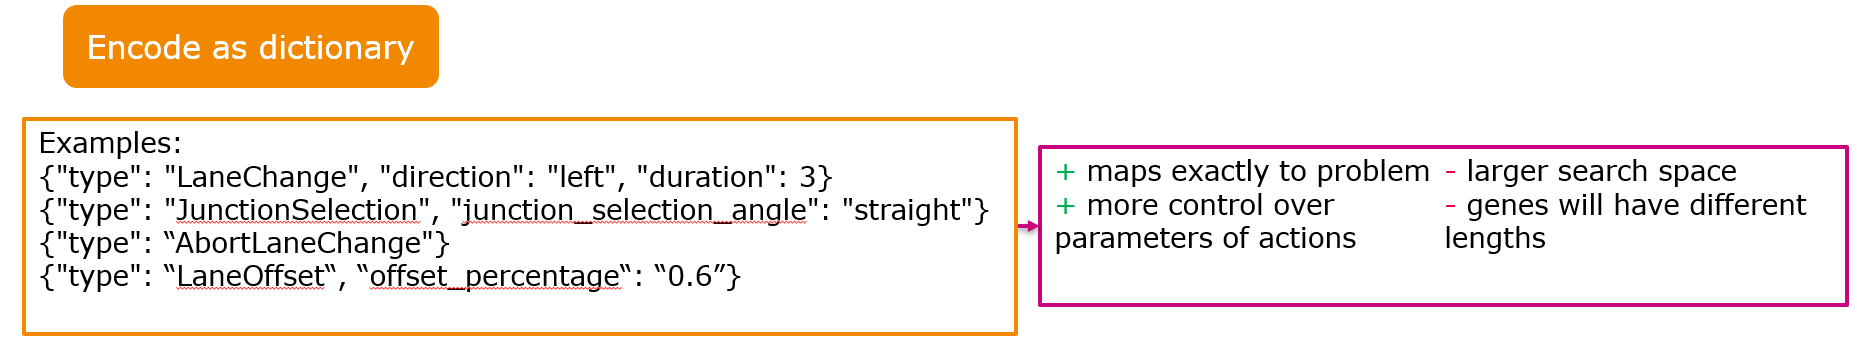
\includegraphics[width=1\linewidth]{figures/dict_encoding}
	\caption{Dictionary}
	\label{figure:encoding:gene:dict}
\end{figure}

\subsection{Cost Function}
\label{implementation:cost_function}
\todo{Suggestion florian: better explain cost values (e.g. 3500 means no emergency break...)}

Cost function is a bit difficult, as we are only using internal values. No ADAS/AD system is tested and we thus have to work with what we got.
This is the code of the cost function:

\begin{lstlisting}[language=Python, tabsize=4]
SEPS_PER_SECOND = 100
# allow emergency breaks to last only 3 seconds
MAX_DURATION = 3 * STEPS_PER_SECOND

cost = 0
duration_counter = 0
for i in range(len(result["ego_emergency_stop"])):
	if not result["ego_emergency_stop"][i]:
		# base cost in case of no current emergency break
		cost = cost + 1
		duration_counter = 0
	else:
		if duration_counter > MAX_DURATION:
			# increase cost if emergency break max duration is exceeded
			cost = cost + 10
		duration_counter += 1
return cost
\end{lstlisting}
result["ego\_emergency\_stop"] is a list with the length $100 * simulation\_duration\_seconds$ (because 100hz). It contains a boolean per step, if the EGO vehicle has initiated an emergency stop.

It would have been interesting to not only test for emergency stops (which will make the NPCs try to get the EGO to hard break often) but also improve time to collison (TTC), as was done by \todo{Ref florian}. However by the time of starting the testing, no working TTC functionality was implemented. Thus, only the emergency break cost function is used by the GA to be optimized.


\section{Behavior Tree}
A behavior tree is a decision tree. \todo{insert a good introduction to BT}
Depending on the functionality under test, it is possible to let the EGO vehicle be controlled by a Behaviour Tree. This makes sense if for example a functionilty like AEB is tested, where only the breaks are controlled. In case of a full driving stack, no Behaviour Tree would be used.

The general idea is to have an EGO vehicle moving in a "relateable" manner trough the world. It will try to dodge standing or slow moving obstacles. This needs to be done in a determinisitc manner in order to no introduce randomness into the simulation.

For this, Behaviour Tree is used. While it has access to the same Action Interface (described in section \ref{implementation:action_interface}) as the Genetic Algorithm, it is more tightly integrated with the Traffic Manger. While the Genetic Algorithm only ingests the results generated by the Simulation with the cost function, the Behaviour Tree needs access to internal functions during the simulation. The following figure shows the behaviour tree implemented.

\iffalse
\begin{figure}[H]
	\centering
	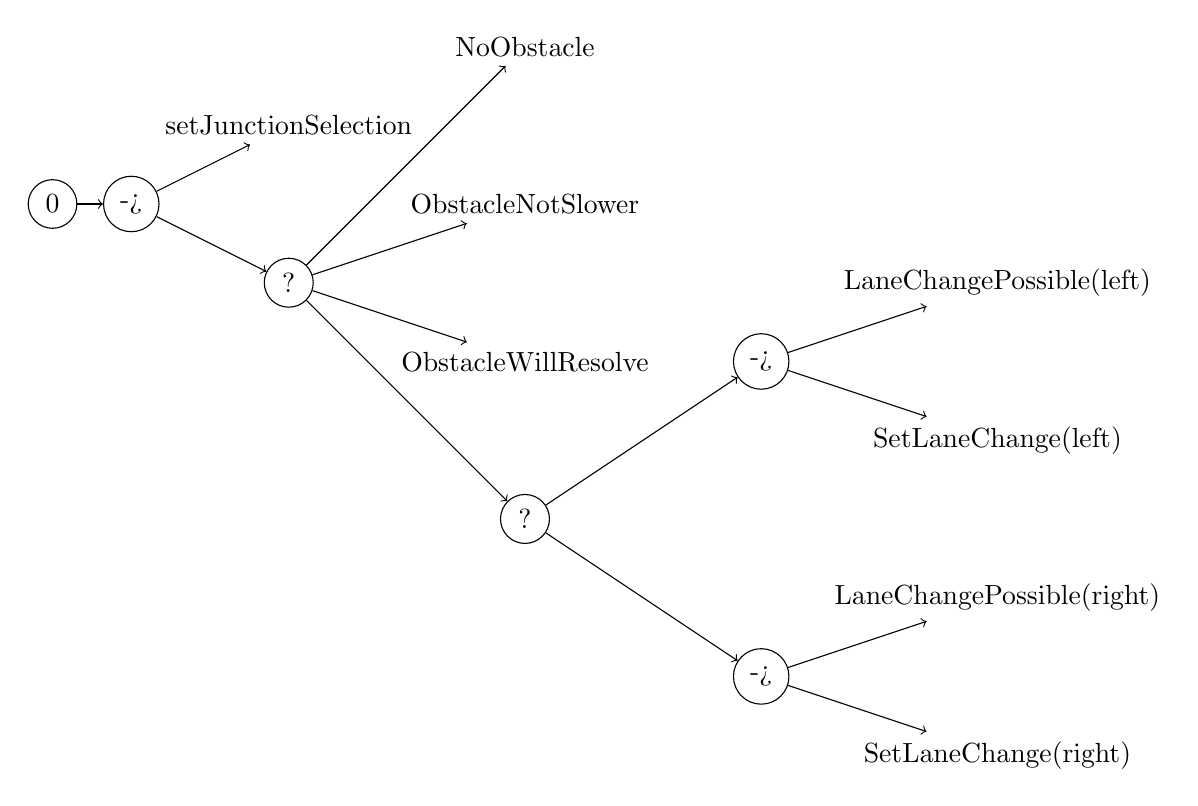
\begin{tikzpicture}
		% Define 1 2 3
		\node[draw, circle] (NodeStart) at (0,0) {0};
		\node[draw, circle] (Sequence1) at (1,0) {->};
		\draw[->] (NodeStart) -- (Sequence1);
		
		\node (Action1) at (3,1) {setJunctionSelection};
		\node[draw, circle] (OR1) at (3,-1) {?};
		\draw[->] (Sequence1) -- (Action1);
		\draw[->] (Sequence1) -- (OR1);

		\node (Action21) at (6,2) {NoObstacle};
		\node (Action22) at (6,0) {ObstacleNotSlower};
		\node (Action23) at (6,-2) {ObstacleWillResolve};
		\node[draw, circle] (OR2) at (6,-4) {?};
		\draw[->] (OR1) -- (Action21);
		\draw[->] (OR1) -- (Action22);
		\draw[->] (OR1) -- (Action23);
		\draw[->] (OR1) -- (OR2);
		
		\node[draw, circle] (Sequence31) at (9,-2) {->};
		\node[draw, circle] (Sequence32) at (9,-6) {->};
		\draw[->] (OR2) -- (Sequence31);
		\draw[->] (OR2) -- (Sequence32);
		
		\node (Action41) at (12,-1) {LaneChangePossible(left)};
		\node (Action42) at (12,-3) {SetLaneChange(left)};
		\node (Action43) at (12,-5) {LaneChangePossible(right)};
		\node (Action44) at (12,-7) {SetLaneChange(right)};
		\draw[->] (Sequence31) -- (Action41);
		\draw[->] (Sequence31) -- (Action42);
		\draw[->] (Sequence32) -- (Action43);
		\draw[->] (Sequence32) -- (Action44);
		
		
	\end{tikzpicture}
	\caption{Used Behaviour Tree}
\end{figure}
\fi

\begin{figure}[ht]
	\centering
	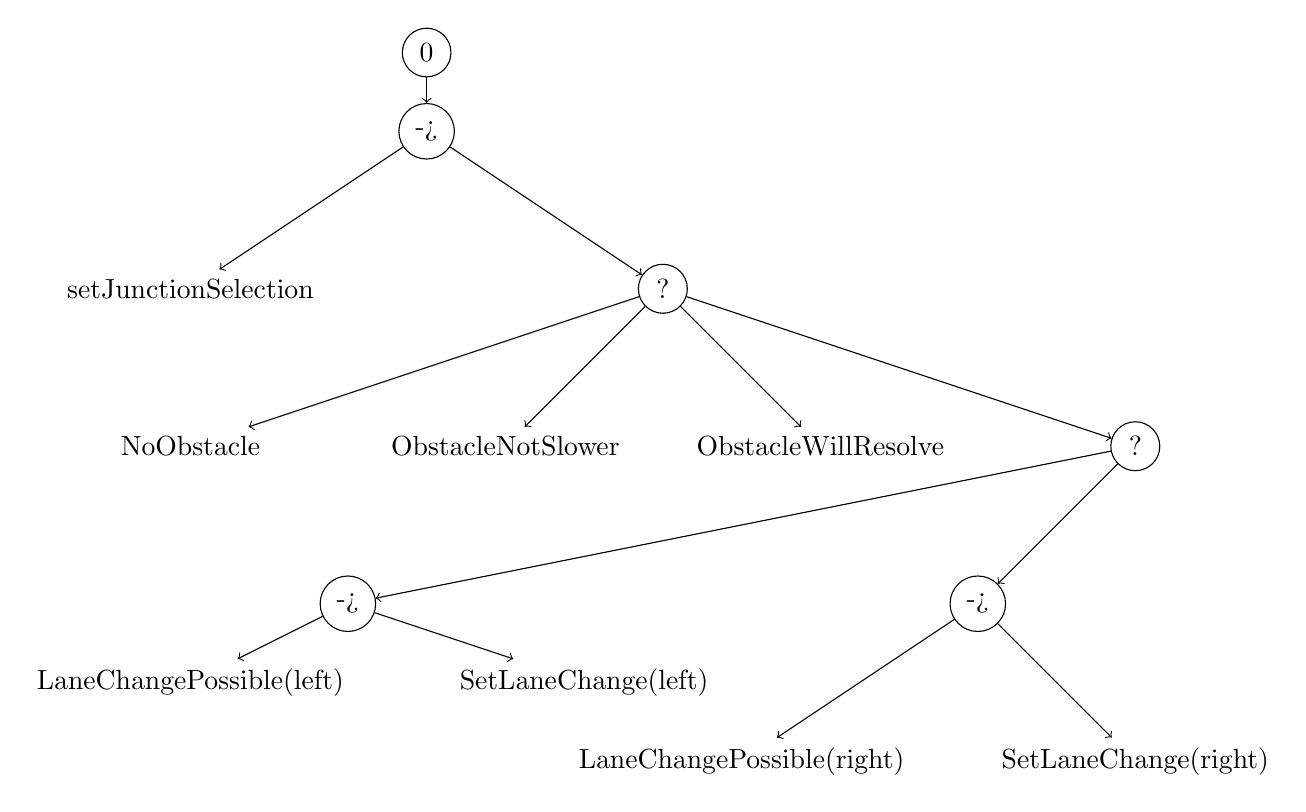
\begin{tikzpicture}
		% Define 1 2 3
		\node[draw, circle] (NodeStart) at (0,0) {0};
		\node[draw, circle] (Sequence1) at (0,-1) {->};
		\draw[->] (NodeStart) -- (Sequence1);
		
		\node (Action1) at (-3,-3) {setJunctionSelection};
		\node[draw, circle] (OR1) at (3,-3) {?};
		\draw[->] (Sequence1) -- (Action1);
		\draw[->] (Sequence1) -- (OR1);
		
		\node (Action21) at (-3,-5) {NoObstacle};
		\node (Action22) at (1,-5) {ObstacleNotSlower};
		\node (Action23) at (5,-5) {ObstacleWillResolve};
		\node[draw, circle] (OR2) at (9,-5) {?};
		\draw[->] (OR1) -- (Action21);
		\draw[->] (OR1) -- (Action22);
		\draw[->] (OR1) -- (Action23);
		\draw[->] (OR1) -- (OR2);
		
		\node[draw, circle] (Sequence31) at (-1,-7) {->};
		\node[draw, circle] (Sequence32) at (7,-7) {->};
		\draw[->] (OR2) -- (Sequence31);
		\draw[->] (OR2) -- (Sequence32);
		
		\node (Action41) at (-3,-8) {LaneChangePossible(left)};
		\node (Action42) at (2,-8) {SetLaneChange(left)};
		\node (Action43) at (4,-9) {LaneChangePossible(right)};
		\node (Action44) at (9,-9) {SetLaneChange(right)};
		\draw[->] (Sequence31) -- (Action41);
		\draw[->] (Sequence31) -- (Action42);
		\draw[->] (Sequence32) -- (Action43);
		\draw[->] (Sequence32) -- (Action44);
		
		
	\end{tikzpicture}
	\caption{Used Behaviour Tree}
\end{figure}


Starting out, \todo{Explain BT}


\chapter{Evaluation}
\label{chap:evaluation}
in this chapter, we evaluate and compare various different settings
In this chapter, we will incrementally move to an optimized Genetic Algorithm


\section{Hyperparameter tuning}
\subsection{Comparing Pop Size}
The mentioned performance limitations forced a lower population size for most simulations than optimal.

\subsection{Different Cost Function}
this will be more tricky to explain as everything is just interal functionality

\subsection{Crossover vs MutProp}
What is the best configuration?

\section{Behaviour Tree enabled}
Will the scenarios be more interesting if the ga is not allowed to have controll over the Ego Vehicle?

\section{Rules enabled}

\chapter{Conclusion}
\section{Test}
Altough lots of shortcommings
Results look very vielversprechend. This thesis hopes to have emphasised that this approach has lots of advanatages

\appendix                       %% closes main document, appendix follows until end; only available in book-classes
\addpart*{Appendix}             %% adding Appendix to tableofcontents

\printbibliography              %% remove, if using BibTeX instead of biblatex
% \include{further_ressources}  %% this is a suggestion: you have to create this file on demand






%%%% end{document}
\end{document}
%% vim:foldmethod=expr
%% vim:fde=getline(v\:lnum)=~'^%%%%\ .\\+'?'>1'\:'='
%%% Local Variables:
%%% mode: latex
%%% mode: auto-fill
%%% mode: flyspell
%%% eval: (ispell-change-dictionary "en_US")
%%% TeX-master: "main"
%%% End:
